%*******10********20********30********40********50********60********70********80

% For all chapters, use the newdefined chap{} instead of chapter{}
% This will make the text at the top-left of the page be the same as the chapter

\chap{Results: The HIV/AIDS Co-authorship Network}
\label{chap:hiv}
%\section{Background}
%After the declaration of the Millenium Challenge Goal 6 in 2000, significant progress has been made in the treatment and prevention of HIV/AIDS, leading to the reverse of related mortality and morbidity. Nevertheless, sub Saharan Africa still carries the burden of HIV/AIDS. For example, in 2009, 2.6 million new cases and 1.8 million of death related to HIV were estimated out of which 68\% and 72\% of respectively new cases and death were in Sub Saharan Africa \cite{joint_united_nations_programme_on_hiv/aids_global_2010}. Even worse, the related deaths attributed to the coinfection of HIV/AIDS and Tuberculosis was estimated at 1.3 million deaths \cite{world_health_organization_global_2010}. In the Republic of Benin, between 2000 and 2013, the impact of the increase in HIV/AIDS research funding has led to an annual decrease of 7.6\%, 1.3\% and 3.1\% respectively in the incidence, the prevalence and the mortality of the disease \cite{joint_united_nations_programme_on_hiv/aids_global_2010,world_health_organization_global_2010}.\\%~\\
%The development of a vaccine to stop the transmission of HIV has proven significantly difficult to develop despite the decades put in research that has not been successful so far \cite{titti_problems_2007,walker_toward_2008}. This is why researchers need to form continuous and sustainable collaboration through intensive network practices that go beyond the regional boundaries \cite{newman_structure_2001}. Scientific collaborations give researchers the opportunity to work and learn from each other. Such collaborations are further needed to overcome the overgrowing challenge of co-infections between HIV/AIDS and Tuberculosis \cite{corbett_growing_2003,gandhi_hiv_2010}.\\%~\\
%Despite the the decades of HIV/AIDS research and the increasing research funding, very little is known on the HIV/AIDS research collaboration network. Successful collaborative research has been essential to the eradication of certain viral illnesses in the past \cite{jamison_disease_2006}. Unfortunately, the extensive research conducted has not prevented HIV from outpacing the proposed solutions. This is a definitive clue to investigating the structure of the HIV/AIDS research community. The provision of evidence based information for Public Health is essential in the formulation of fundamental principles and guidelines. Research collaboration constitutes an important tool to achieving such goals.  This is why we propose in this chapter, to document, describe and analyze the different aspects of the HIV/AIDS research collaboration in the Republic of Benin.\\
%Understanding the structure of this network is capital since it can help improve research prioritization \cite{ghafouri_social_2014}, identify prolific researchers, better design, strategic planning and implementation of research programs \cite{morel_co-authorship_2009}, and promote cooperation and translational research initiatives \cite{gonzalez-alcaide_scientific_2012}. We choose a social network analysis approach which will reveal undiscovered knowledge on effort of researchers in working together towards the reduction of the burden of HIV/AIDS in Benin. 
%Our study focuses on the Network analysis of the scientific collaborations through co-authorship network analysis.

\section{Data}
\label{sec:hiv_data}
The literature search was conducted in the Web Of Science (WOS) using combinations of HIV/AIDS related MeSH terms including "HIV", "AIDS", "VIH" and "HIV Infections". 
%We restricted the search to the period from 1996 to 2016 and to "Benin" for country. We further screened the papers in order to only select those published by Beninese authors, or papers published on HIV/AIDS from Benin. No restriction was placed upon the document types.  We first started querying with each term independently, we then combined the other terms so the query return the maximum number of results. The  Full citations information containing the authors' names, their institutional affiliations, the year of publication, as well as the number of times the document was cited were recorded as a bibliographic corpus in text format. After a second screening only research that have met the above listed inclusion criteria and that were published between January 1, 1996 and December 31, 2016 were selected.\\
The final query set (Table \ref{table: hiv_search}) returned 237 records. After a rigorous screening process, 102 documents met the selection criteria. On average, there were 9.47 authors per published document.

\begin{table}[h!]
\caption{HIV/AIDS Bibliographic Search Queries.}
\label{table: hiv_search}
\centering
\hspace*{-0.25cm}
\footnotesize
\begin{tabular}{llc}
\toprule
Set & \multicolumn{1}{c}{Queries} & Results \\
\midrule
\#1 & TOPIC: (HIV AIDS) Refined by: COUNTRIES/TERRITORIES: (BENIN) & 52 \\\\
\#2 & TOPIC: (HIV AIDS) AND ADDRESS: (BENIN) & 107 \\\\
\#3 & \begin{tabular}[c]{@{}l@{}}TOPIC: (HIV) OR TOPIC: (AIDS) AND ADDRESS: (BENIN),\\Refined by:COUNTRIES/TERRITORIES: (BENIN)\end{tabular} & 182 \\\\
\#4 & \begin{tabular}[c]{@{}l@{}}TOPIC: (HIV) OR TOPIC: (VIH) OR TOPIC: (AIDS) AND ADDRESS: (BENIN),\\Refined by: COUNTRIES/TERRITORIES: (BENIN)\end{tabular} & 182 \\
\midrule
Final Set & \#1 OR \#2 OR \#3 OR \#4 & 237\\
\bottomrule
\end{tabular}
\end{table}

The Author Name Disambiguation process led to the identification of 516 unique authors with a precision of 99.88\% and a recall of 82.54\%. The generated multigraph co-authorship network therefore contained 516 vertices (authors) and 5,114 parallel edges (collaborations). The number of unique authors for HIV research is roughly one third of the Malaria ones. As displayed in figure \ref{hiv_pubDist}, we can see the significant increase in publications, scientific collaborations and the number of authors involved in HIV/AIDS research from 2008 until 2016. This general upward trend seems to be linear from the year 2008 to 2016. The variation seen between adjacent years may reflect the  relatively small productivity of HIV research prior to the year 2008.

\begin{figure}[h!]
\centering
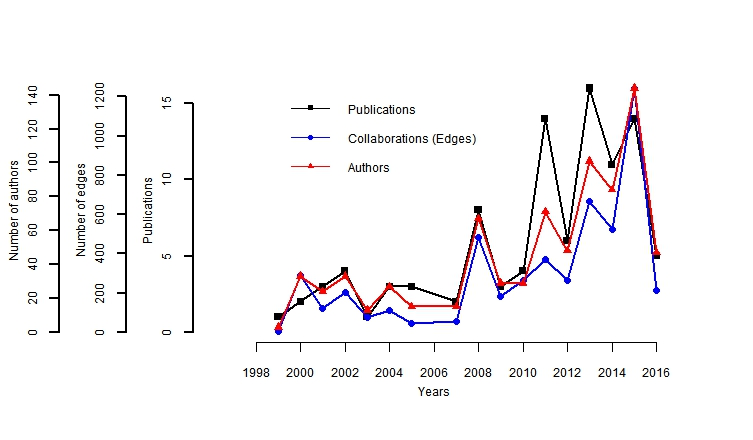
\includegraphics[scale=0.65]{Chapters/hiv/pubDist}
\caption{Evolution of the published HIV related documents, authors and collaborations from January 1996 to December 2016}
\label{hiv_pubDist}
\end{figure}

\section{Descriptive Data Analysis}
\label{sec:hiv_descstat}
For the multigraph network, the degree distribution varies between 1 and 403 with an average degree distribution of 19.82 and a median of 12. In addition, there was a substantial number of vertices with low degrees (Fig. \ref{hiv_fig1}). The log scale distribution of the degrees on figure \ref{hiv_fig2} reveals that there was also a non-trivial number of vertices with higher order of degree magnitudes. There is a tendency of the vertex degrees to follow a heavy-tail distribution suspected on figure \ref{hiv_fig1}.

\begin{figure}[h!]
\centering
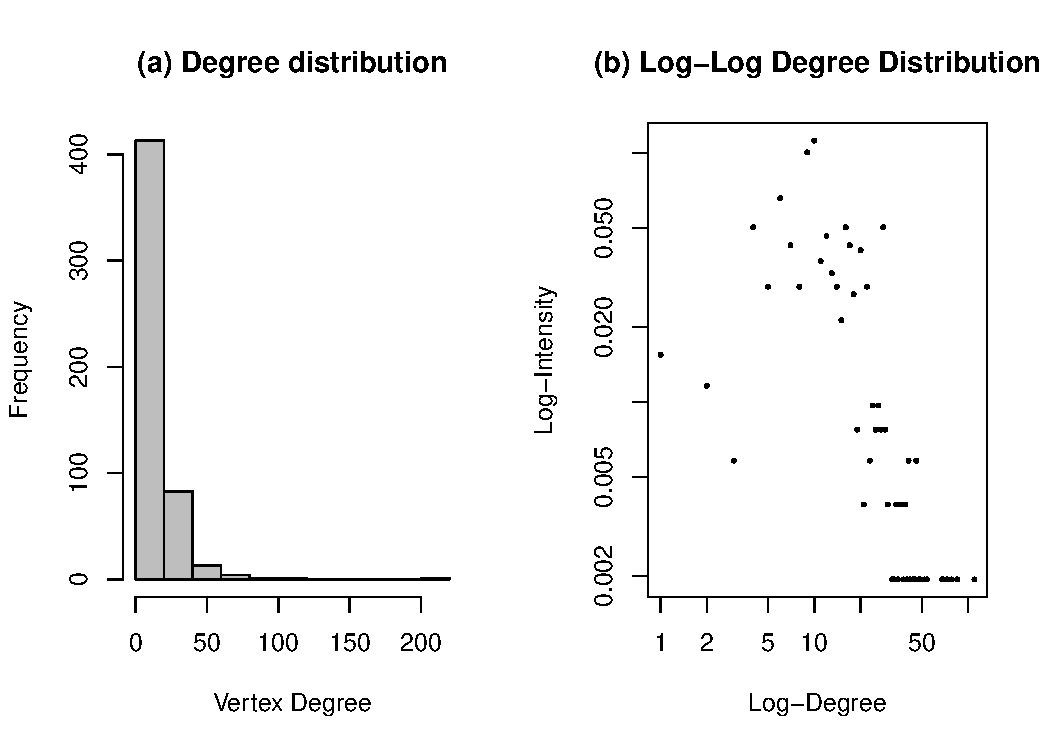
\includegraphics[scale=0.65]{Chapters/hiv/degreeDistribution}
\caption{Degree distribution of the HIV/AIDS co-authorship network}
\label{hiv_fig1}
\end{figure}

After we convert the multigraph network in a weighted graph, it results in a simple graph of 516 vertices and 3,966 weighted edges. Closeness centrality measures range between $3.76\times 10^{-6}$ and $3.19\times 10^{-5}$ with a median of $3.13\times 10^{-5}$. Betweenness measures range between 0 and 49,280 with a median of 426.2. A network visualization with the vertices' size proportional to betweenness centrality measures clearly reveals the presence of broker authors (Figure \ref{hiv_fig5} and Table \ref{table: hiv_list}). The median Eigenvectors is 0.202 with a mean of 0.045. The eigenvectors measures confirm the presence of author hubs in the network suggesting the presence of closed collaboration groups. Table \ref{table: hiv_list} presents a list of the 10 author hubs with the highest Eigenvectors values.

\begin{figure}[h!]
\centering
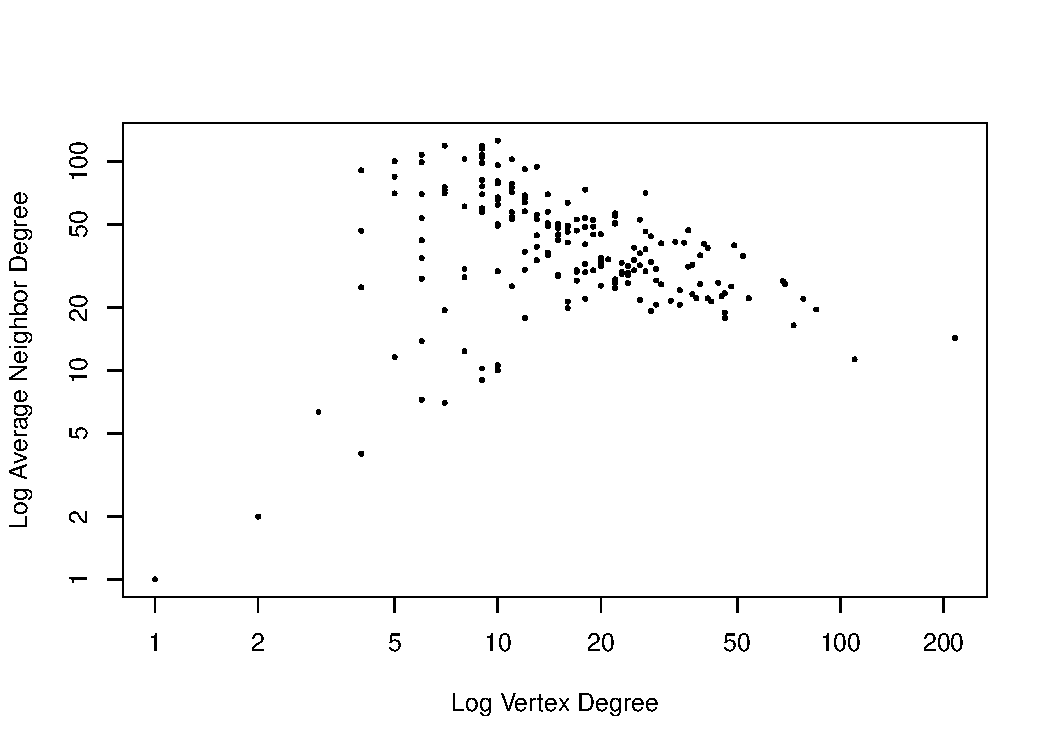
\includegraphics[scale=0.65]{Chapters/hiv/logAvgDegree}
\caption{Log-Average Neighbor degree Distribution of the HIV/AIDS co-authorship network}
\label{hiv_fig2}
\end{figure}

Edge betweenness centrality measures identify co-authorship collaboration ties that are important for the flow of information. Table \ref{table: hiv_list} presents the top 10 most important collaboration ties for the flow of information in the HIV/AIDS co-authorship network in Benin.

\begin{table}[h!]
\caption{List of the most important authors and collaborations in the HIV/AIDS co-authorship network}
\label{table: hiv_list}
\centering \footnotesize
\begin{tabular}{l}
  \toprule
\textbf{Top 10 Brokers}\\
%\hline
\hspace{20pt}ZANNOU DJIMON MARCEL\\
\hspace{20pt}ALARY MICHEL\\
\hspace{20pt}LEROY VALERIANE\\
\hspace{20pt}AZONDEKON ALAIN\\
\hspace{20pt}ANAGOUNOU SEVERIN\\
\hspace{20pt}ADE GABRIEL\\
\hspace{20pt}AZONKOUANOU ANGELE\\
\hspace{20pt}NDOYE IBRA\\
\hspace{20pt}NDOUR MARGUERITE\\
\hspace{20pt}AFFOLABI D\\
\hline
\textbf{Top 10 most connected authors (Top 10 network hubs)}\\
\hspace{20pt}ZANNOU DJIMON MARCEL\\
\hspace{20pt}ALARY MICHEL\\
\hspace{20pt}ANAGOUNOU SEVERIN\\
\hspace{20pt}LOWNDES CATHERINE M\\
\hspace{20pt}LABBE ANNIECLAUDE\\
\hspace{20pt}DABIS FRANCOIS\\
\hspace{20pt}MINANI ISAAC\\
\hspace{20pt}BEHANZIN LUC\\
\hspace{20pt}DIABATE SOULEYMANE\\
\hspace{20pt}EKOUEVI DIDIER K\\
\hline
\textbf{Top 10 most important edges for information flow}\\
\hspace{20pt}ZANNOU DJIMON MARCEL -- LEROY VALERIANE\\
\hspace{20pt}ZANNOU DJIMON MARCEL -- NDOUR MARGUERITE\\
\hspace{20pt}ALARY MICHEL -- AZONKOUANOU ANGELE\\
\hspace{20pt}ZANNOU DJIMON MARCEL -- NDOYE IBRA\\
\hspace{20pt}ANAGOUNOU SEVERIN -- ADE GABRIEL\\
\hspace{20pt}ZANNOU DJIMON MARCEL -- WACHINOU ABLO PRUDENCE\\
\hspace{20pt}ZANNOU DJIMON MARCEL -- DALMEIDA MARCELLINE\\
\hspace{20pt}AZONDEKON ALAIN -- ADE GABRIEL\\
\hspace{20pt}AZONKOUANOU ANGELE -- AZONDEKON ALAIN\\      
\hspace{20pt}ZANNOU DJIMON MARCEL -- COFFIE PATRICK A\\
\hline
\textbf{Weak articulation points}\\
\hspace{20pt}ATADOKPEDE FELIX\\
\hspace{20pt}NDOUR MARGUERITE\\
\hspace{20pt}DALMEIDA MARCELLINE\\
\hspace{20pt}AZONDEKON ALAIN\\
\hspace{20pt}GANDAHO PROSPER\\
\hspace{20pt}AFFOLABI D\\
\hspace{20pt}ADE GABRIEL\\
\hspace{20pt}ZANNOU DJIMON MARCEL\\
\bottomrule
\end{tabular}
\end{table}

\subsection{Network Cohesion}
In total, 29 maximal cliques were detected in the network among which 2 cliques of size 24, 1 clique of size 23 and 4 cliques of size 3. Larger maximal cliques sizes range from 14 authors to 25 authors. \\The HIV/AIDS co-authorship network has a density of 0.0298 indicating that the baseline probability of collaboration tie formation is 2.98\%. The network also has a transitivity of 0.482 meaning that 48.2\% of the connected triples in the network are close to form triangles. The transitivity metrics is a measure of the global clustering of the network.\\The network is not connected and a census of all the connected components within the network reveals the existence of a giant component that dominates all the other connected components. The giant component of the HIV/AIDS co-authorship network includes 88.6\% (457 vertices) of all the vertices in the network with the other components alone carrying less than 1\% of the vertices (Fig. \ref{hiv_fig5}). \\
Information flow assessment of this network via cut vertices confirms the existence of 8 authors as the most vulnerable vertices in the network. Table \ref{table: hiv_list} lists the authors that constitute the weak articulation points in the HIV/AIDS co-authorship network. The identification of cut vertices is a measure of the vulnerability of the HIV/AIDS co-authorship network \cite{kolaczyk_statistical_2014}.\\
Via the agglomerative hierarchical clustering method, we identify 24 different research communities (or clusters) which sizes range between 1 and 108 authors. Large research communities contain between 71 and 108 authors. Medium size research communities contain between 10 and 55 authors. Out of the 24 clusters detected, 12 are part of the giant component. Figure \ref{hiv_fig5} displays the structure of the network with each different colors representing each of the 24 clusters.

\begin{figure}[h!]
\centering
\hspace{-1.5cm}
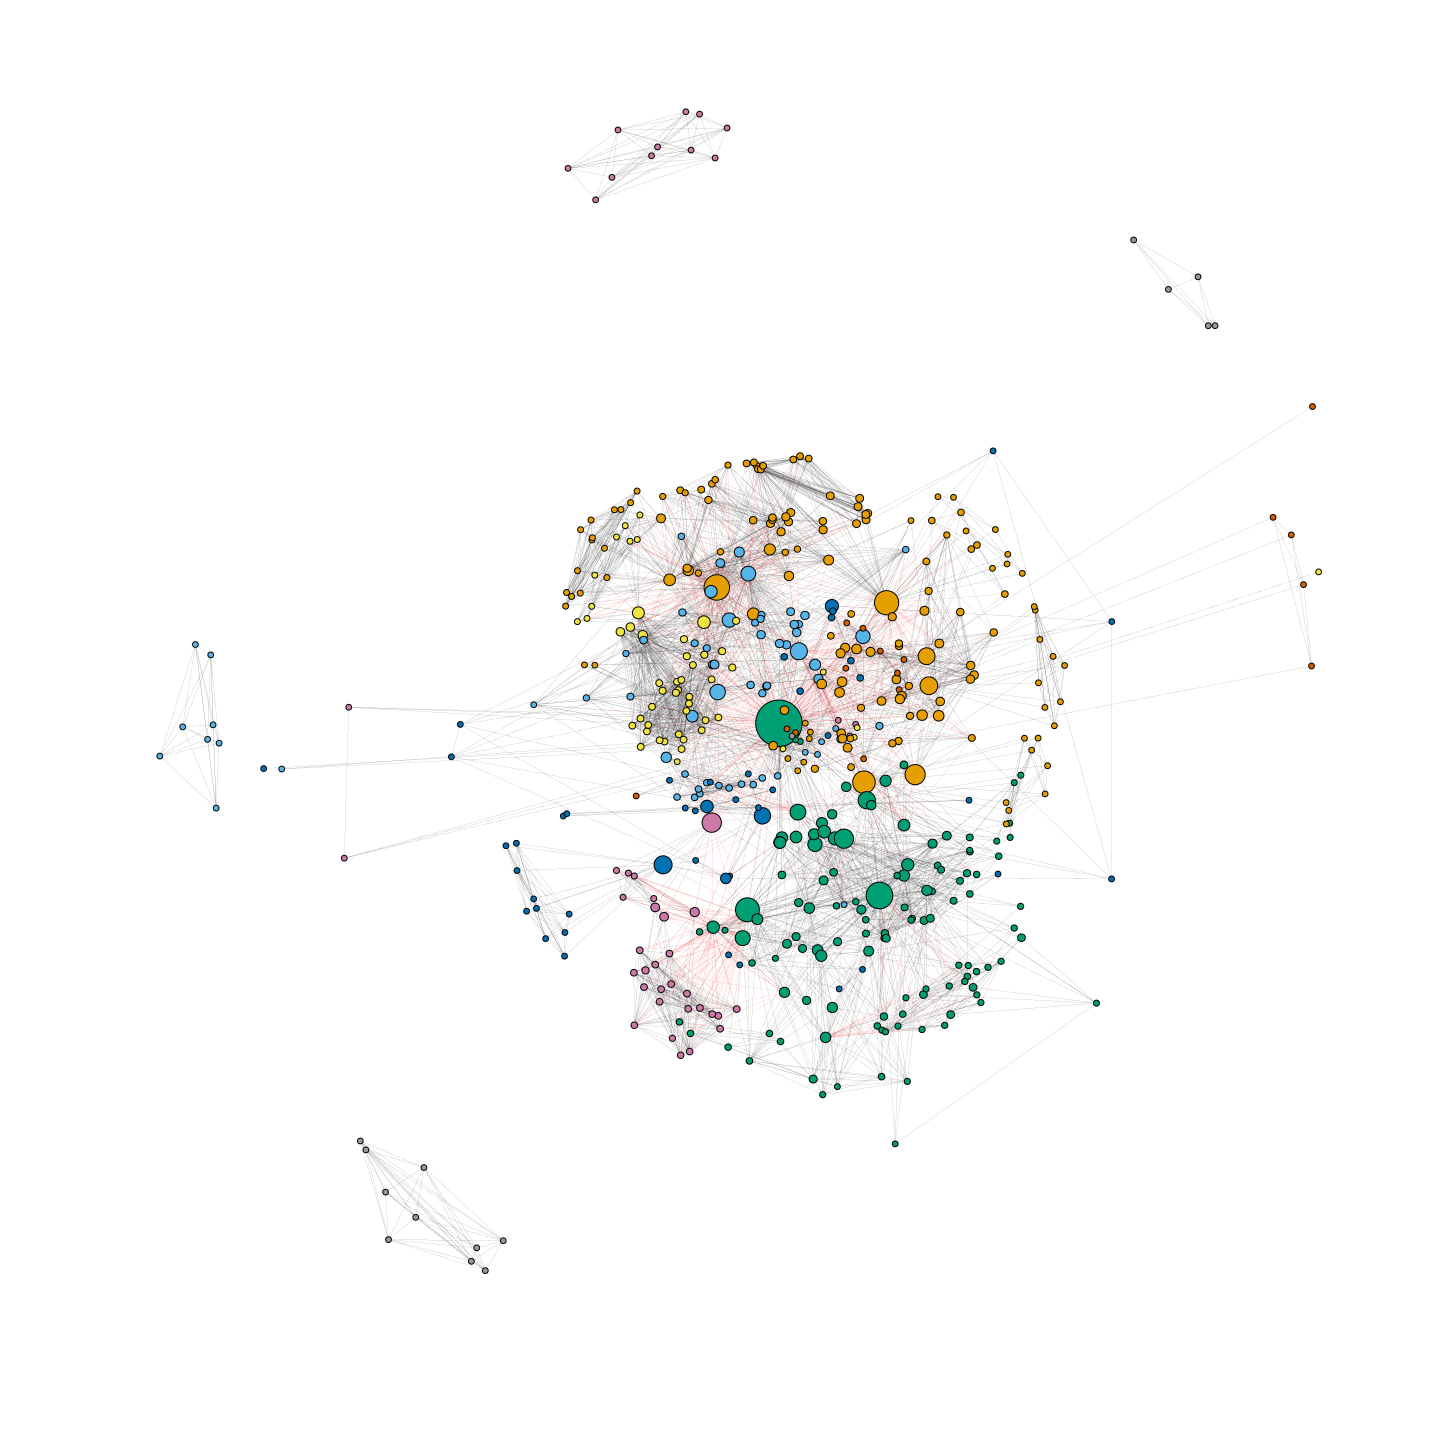
\includegraphics[scale=0.45]{Chapters/hiv/hivaids_net}
\caption{Topological Structure of the HIV/AIDS co-authorship network. Authors (vertices) of the same color belong to the same research community or cluster}
\label{hiv_fig5}
\end{figure}

%\pagebreak
\section{Modeling}
\subsection{Mathematical Modeling}
We performed 1,000 Monte Carlo based simulations to test the significance of the observed characteristics of the HIV/AIDS co-authorship network. Figure \ref{hiv_fig3} clearly demonstrates that the number of communities detected is unusual from the perspective of both Classical random graphs and generalized random graphs (p-value < 0.0001). From the Classical random graph model, the expected number of communities was 5.574 (95\%CI: 5.53 -- 5.62). Similarly, the expected number of communities from the generalized random graph model is 6.65 (95\%CI: 6.60 -- 6.70).

\begin{figure}%[h!]
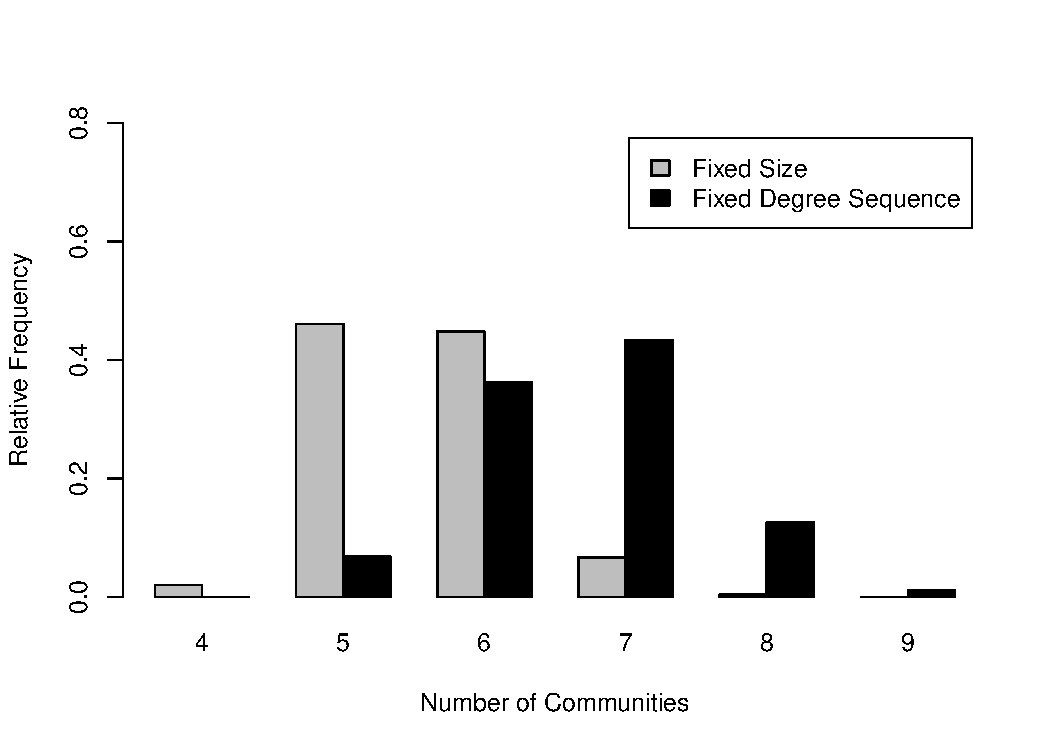
\includegraphics[scale=0.65]{Chapters/hiv/randomComm}
\centering
\caption{Monte-Carlo simulations of the HIV/AIDS network: Number of detected communities by the random graph models}
\label{hiv_fig3}
\end{figure}
Figure \ref{hiv_fig4} displays the number of detected research communities using the Barab\'asi-Albert's preferential attachment and the Watts-Strogatz models. The observed number of communities was extreme per both models (p-value < 0.0001). The expected number from the Watts-Strogatz model simulations is 3.181 (95\%CI: 3.16 -- 3.21) and 22.8 (95\%CI: 22.7 -- 23.0) from the Barab\'asi-Albert model simulations. 
We also compared the clustering coefficient and the average shortest-path length. Let's recall that the observed clustering coefficient is 0.482. On one hand, there was substantially more clustering in our HIV/AIDS co-authorship network than expected from both random graph models (p-value < 0.0001). The expected clustering coefficients was 0.0365 (95\%CI: 0.0363 -- 0.0365) and 0.0842 (95\%CI: 0.0841 -- 0.0843) respectively for the classic random graph and the generalized random graph models.\\
On the other hand, there was substantially less clustering in our HIV/AIDS co-authorship network than expected by the Watts-Strogatz Small World model which expected clustering was 0.72615 (95\%CI: 0.72611 -- 0.72618).

\begin{figure}[h!]
\centering
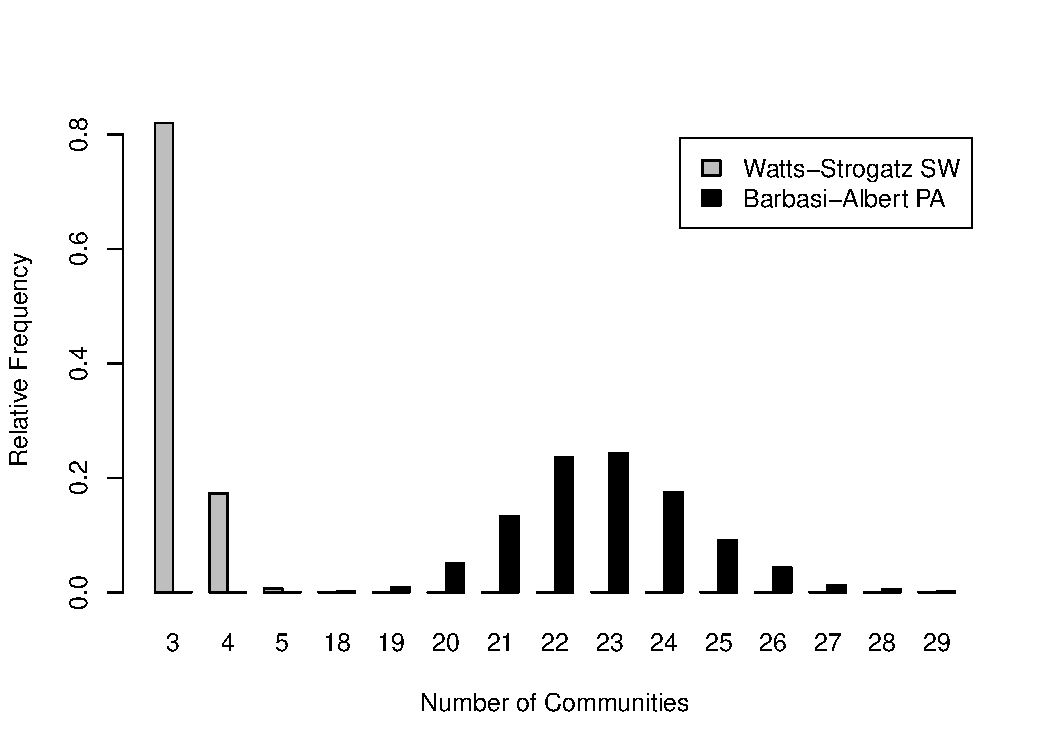
\includegraphics[scale=0.65]{Chapters/hiv/mechanisticComm}
\caption{Monte-Carlo simulations of the HIV/AIDS network: Number of detected communities by the Watts-Strogatz and the Barab\'asi-Albert models}
\label{hiv_fig4}
\end{figure}

We observed an average shortest-path length of 2.75 in the HIV/AIDS co-authorship network. This observed shortest-path length is significantly larger than what was expected from the random graph models (p-value < 0.0001) and significantly lower than what was expected from Watts-Strogatz small world model and the Barab\'asi-Albert preferential attachment model (p-value < 0.0001).\\The average shortest-path length was 2.49069 (95\%CI: 2.49062 -- 2.49077) and 2.381 (95\%CI: 2.380 2.381) respectively for the classic random graph and the generalized random graph models.\\For the Watts-Strogatz small world and the Barab\'asi-Albert preferential attachment models, the average shortest-path length is respectively 5.31 (95\%CI: 5.28 -- 5.36) and 7.35 (95\%CI: 7.31 -- 7.38).\\~\\
We performed the same simulations on the giant component of the network with similar results leading to similar outcomes.
\pagebreak
\subsection{Statistical Modeling}
%For the purposes of modeling the temporal dynamic of collaboration tie formation, we subset the network in different temporal snapshots. We subset the network, generating snapshots in a certain way that balanced the number of edges across the years. Such an uneven subsetting improved the robustness of our models and ensured model convergence. We ended up with 7 snapshots representing respectively the following timestamps: 1996 -- 2006, 2007 -- 2009, 2010 -- 2011, 2012 -- 2013, 2014, 2015 and 2016. %\\
%Figure \ref{fig:hiv_dynNetwork} displays the topological structure of the snapshots of the different time steps.

\subsubsection{Stochastic Block Model}
\label{sec:hiv_results_sbm}
The SBM identifies 26 classes with a degree of latitude of 17 to 26 classes being reasonable (See ICL plot on figure \ref{fig:hiv_sbmgof}).

\begin{figure}[h!]
\centering
\hspace*{-1cm}
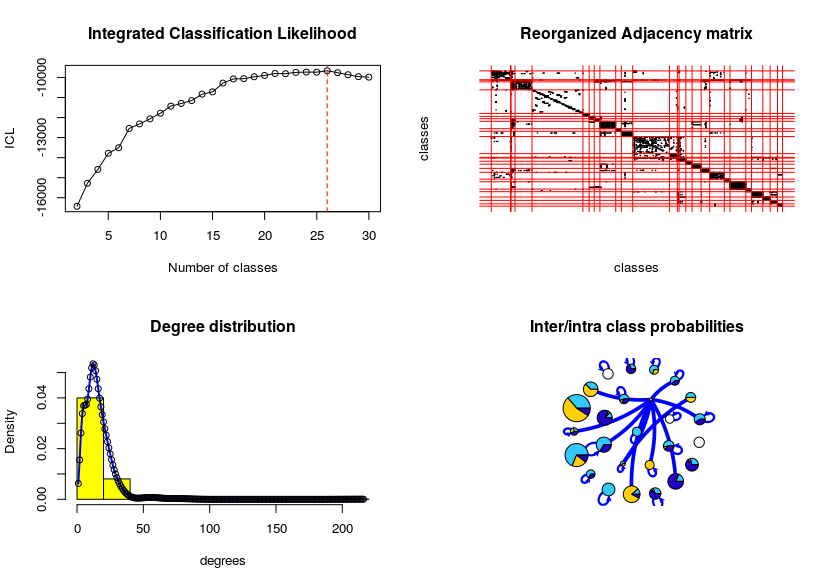
\includegraphics[scale=0.85]{Chapters/hiv/statMod/hiv_sbm}
\caption{Summary of the goodness-of-fit of the SBM analysis on the HIV/AIDS co-authorship network.}
\label{fig:hiv_sbmgof}
\end{figure}

Regarding the degree distribution, the fitted SBM describes well the observed degree distribution. On the network depicting the inter/intra probabilities between the classes, the vertices represent the 26 identified classes, with each one of them divided into a pie chart displaying the proportion of authors of international affiliations (lightblue), authors of regional or other African affiliations (darkblue), and authors affiliated to Beninese research institutions (yellow). Generally, the dominance across the classes of international and regional players is observed. In addition, we observe denser ties between medium size and smaller size classes. \\
A close examination of the pie charts reveals that almost all the classes are heterogeneous. We note the presence of 2 large classes which are classes 5 and 12 (See reorganized adjacency matrix on figure \ref{fig:hiv_sbmgof}). Class 5 is dominated by researchers with Beninese affiliations but appears sparser than class 12 which is dominated by international authors (Figure \ref{fig:hiv_sbmgof}). \\

\begin{figure}[h!]
\centering
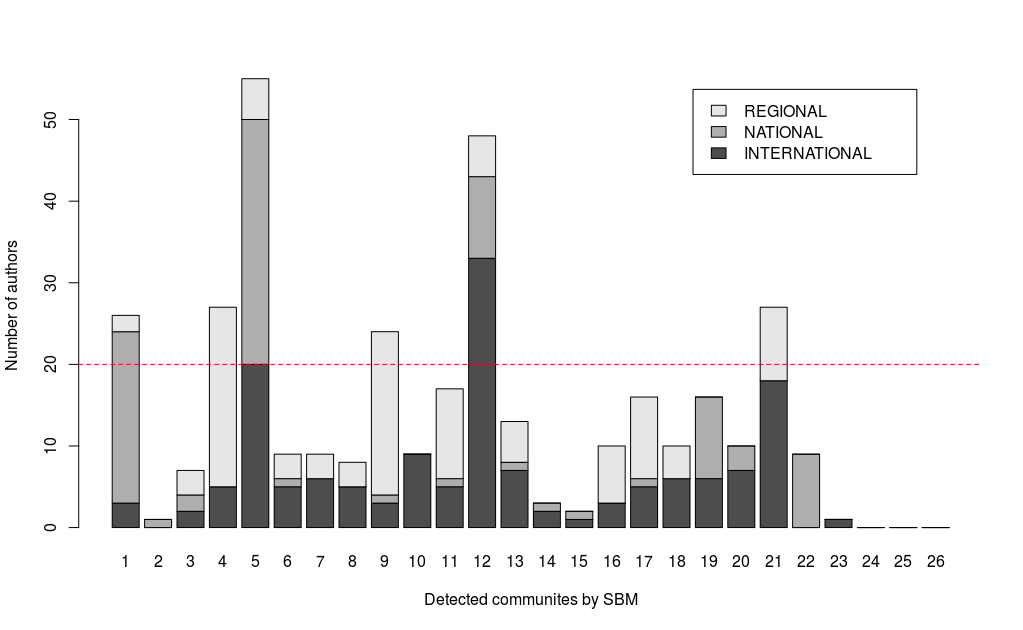
\includegraphics[scale=0.5]{Chapters/hiv/statMod/hiv_sbm_barplot}
\caption{Distribution of national, international and regional authors by communities detected by the SBM in the HIV/AIDS network.}
\label{fig:hiv_sbmdist}
\end{figure}

On figure \ref{fig:hiv_sbmgof2}, we present the SBM results emphasizing the largest classes (with more than 20 members). Here, we can confirm that smaller classes tend to collaborate more among themselves and intra-class collaborations tend to occur more.

\begin{figure}[h!]
\centering
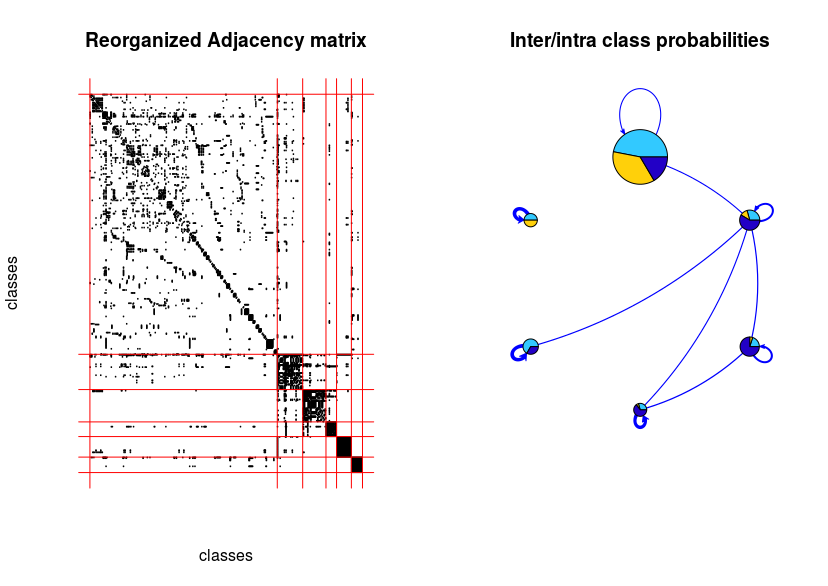
\includegraphics[scale=0.65]{Chapters/hiv/statMod/hiv_sbm2}
\caption{Summary of the goodness-of-fit of the SBM analysis highlighting interactions between the largest classes of the HIV/AIDS co-authorship network.}
\label{fig:hiv_sbmgof2}
\end{figure}

\pagebreak
\subsubsection{Exponential Random Graph Model}
\label{sec:hiv_results_ergm}
Different models were fit with the ERGM method (Table \ref{tab:hiv_ergm}). Model 1, the null model, contains only the "edge" term. The inverse logit of the coefficient associated with this term is $0.0298$ which is the baseline probability of collaboration ties establishment and also the density of the HIV/AIDS co-authorship network.

\begin{table}
\begin{center}
\hspace*{-1cm}
\small
\begin{tabular}{@{}lcclclcl@{}}
\toprule
           &  & Model 1 &  & Model 2  &  & Model 3\\ \cmidrule{3-3} \cmidrule{5-5} \cmidrule{7-7}            &  & Estimate ($SE$) &  & Estimate ($SE$)  &  & Estimate ($SE$) \\ \midrule
           Network structural predictor &  &   &  &  &  \\
\hspace{10pt}Intercept(edge) & & $-3.48 \; (0.02)^{***}$ & & $-7.51 \; (0.06)^{***}$ & & $-7.55 \; (0.07)^{***}$ \\ \\
Number of times cited        & &       --  & & $\hspace{6pt}0.00 \; (0.00)^{***}$ &  & $\hspace{6pt}0.00 \; (0.00)^{***}$  \\
Number of collaborations     & &  --  & & $\hspace{6pt}0.08 \; (0.00)^{***}$ &  & $\hspace{6pt}0.08 \; (0.00)^{***}$  \\
Number of publications       & &  --  & & $-0.29 \; (0.01)^{***}$ & & $-0.28 \; (0.01)^{***}$ \\
Homophily on cluster assignment &  &   --  &  & $\hspace{6pt}5.01 \; (0.05)^{***}$ &  & $\hspace{6pt}5.02 \; (0.05)^{***}$  \\
Homophily on collaboration type   &   & -- &   & $\hspace{6pt}0.77 \; (0.05)^{***}$ &  & $\hspace{6pt}0.72 \; (0.05)^{***}$  \\ \\
Factor attribute effect (collaboration type) &  &    &  &  &   &   \\
\hspace{10pt}International   &  & --   &  & --   &  & $REF$\\
\hspace{10pt}National        & &  --   &  &  -- & & $-0.05 \; (0.04)^{~~~~}$       \\
\hspace{10pt}Regional        & &  --   &  & --  & & $\hspace{6pt}0.21 \; (0.03)^{***}$  \\ \\
\midrule
AIC     & & $\hspace{6pt}35668.54$ &  & $\hspace{6pt}18956.20$   & & $\hspace{6pt}18912.74$   \\
BIC     & & $\hspace{6pt}35678.34$ &  & $\hspace{6pt}19014.98$   & & $\hspace{6pt}18991.12$  \\
Log Likelihood               & & $-17833.27$ & & $-9472.10$   & & $-9448.37$   \\
\bottomrule
\multicolumn{4}{l}{\scriptsize{$^{***}p<0.001$, $^{**}p<0.01$, $^*p<0.05$}}
\end{tabular}
\caption{ERGM of the HIV/AIDS co-authorship network.}
\label{tab:hiv_ergm}
\end{center}
\end{table}

In model 2, we included all nodal variables, a homophily term on collaboration type and on cluster assignment determined from the SBM. Model 2 improved tremendously compared to model 1 (See AIC, BIC and model likelihood in table \ref{tab:hiv_ergm}). We note a decrease in the edge effect (Coefficient $=-7.51$, $p<0.001$) with the associated conditional probability (given all the other terms in the model) estimated at $0.05\%$. For the remaining terms in model 2, we observed a positive and significant effect except for the number of publications. Model 3 differs from model 2 in that it includes a factor term on the collaboration type with a substantial improvement compared to model 2. Model 3 is therefore chosen as our last model. Regarding the number of publication, a one unit increase in the number of publication is associated with $32.3\%$ average decrease in the odds of collaboration ties establishment. Model 3 further proves that the process underlying the structure of the HIV/AIDS co-authorship network in Benin is mainly driven by homophily on cluster assignment or membership to a research community or group (Coefficient $=5.02$, $p<0.001$). The conditional probability of any two authors belonging to the same research group to collaborate is estimated at $7.38\%$ compared to the baseline probability of $2.98\%$. The same probability changes to $14.06\%$ after adjustment by the collaboration type, and $11.82\%$ after adjusting for the number of citations, collaborations and publications. Compared to researchers affiliated to international institutions, researchers affiliated to Beninese institutions have $5.1\%$ average decrease in the odds of collaboration tie establishment. This average decrease is not statistically significant ($p>0.05$). For researchers affiliated to institutions other than Beninese institutions, the odds of collaboration tie establishment increases on average by $18.9\%$ compared to internationally affiliated researchers. Overall, model 3 estimated the probability of collaboration tie formation at $11.8\%$ for international researchers, $11.3\%$ for national researchers and $14.2\%$ for regional players. \\
Since none of the models containing endogenous ERGM terms and/or the dyadic variables, attained convergence, we do not present those results in table \ref{tab:hiv_ergm}.

\begin{figure}[!h]
\centering
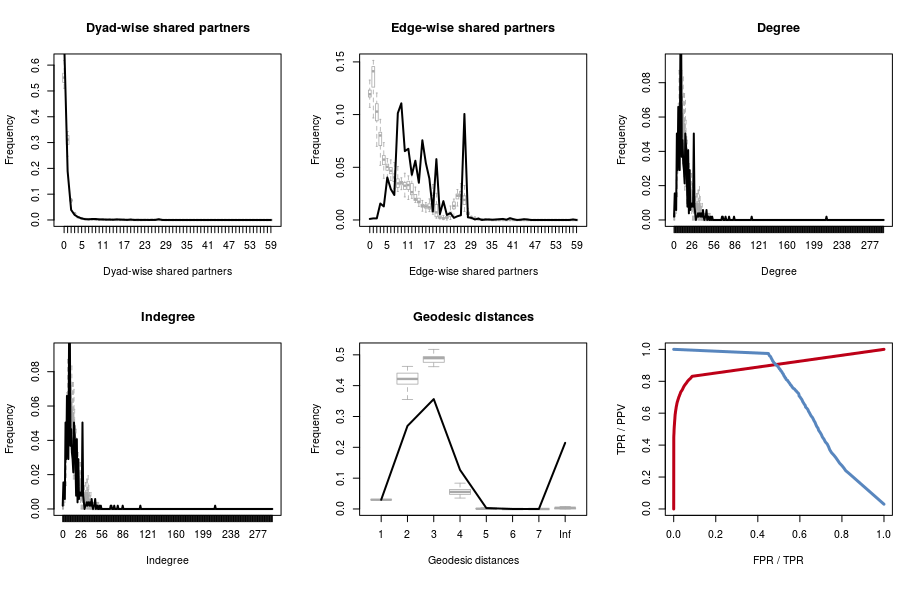
\includegraphics[scale=0.65]{Chapters/hiv/statMod/ergm_gof2}
\caption{ERGM goodness-of-fit of final model 3 assessment on the HIV/AIDS co-authorship network.%\\
%The observed properties are depicted by the black lines. Gray lines with circles represent the 95\% confidence intervals for the simulated network properties. Goodness-of-fit is asserted when the black lines lie in-between the confidence intervals lines.
}
\label{fig:hiv_ergm-gof}
\end{figure}

Figure \ref{fig:hiv_ergm-gof} presents the goodness-of-fit of the final model 3. It appears that the ERGM fits well the observed HIV/AIDS co-authorship network in terms of edge-wise, dyad-wise shared partners, degree, geodesic distances, triad census. In addition, $89.9\%$ of the time, model 3 accurately predicted new collaboration ties among the authors ($AUC=89.9\%$, random models light curves not displayed).

\subsubsection{Temporal Exponential Random Graph Model}
\label{sec:hiv_results_tergm}
We subset the cumulative observed network in six snapshots according to the following time spans: 1996 -- 2001, 2002 -- 2008, 2009 -- 2010, 2011 -- 2012, 2013 -- 2014 and 2015 -- 2016. In figure \ref{fig:hiv_dynNetwork}, we show the topological structure of the network snapshots for the different time steps.

\begin{figure}[!ht]
\hspace{-1.25cm}
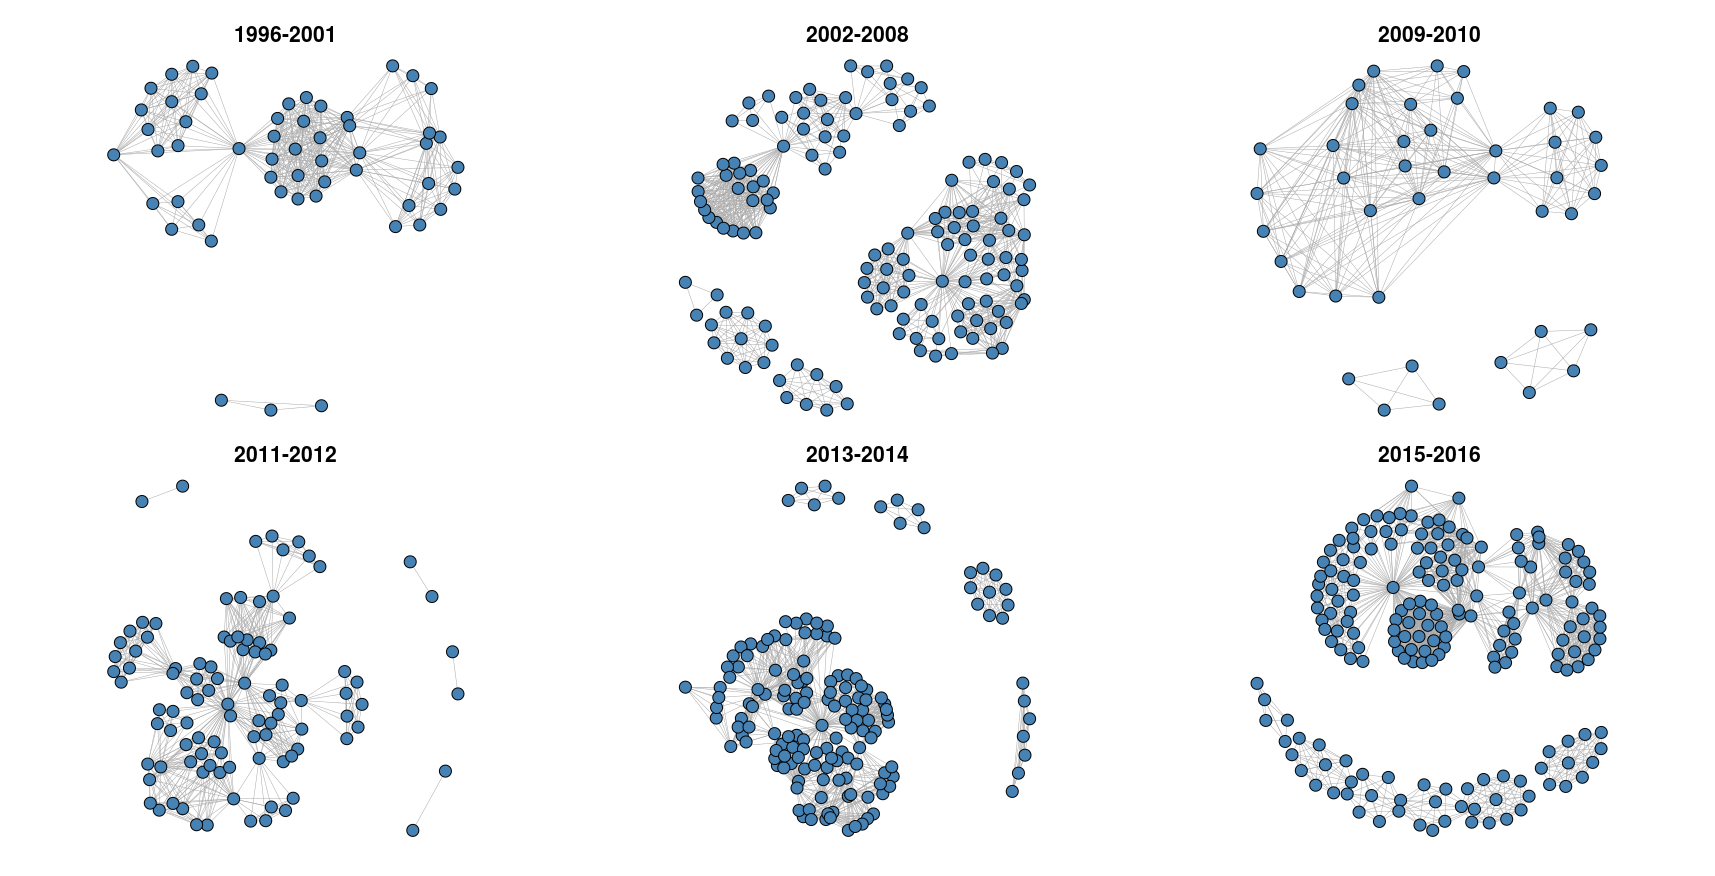
\includegraphics[scale=0.4]{Chapters/hiv/statMod/hiv_dynNetwork}
\caption{Topological structure of the different snapshots of the HIV/AIDS co-authorship network.}
\label{fig:hiv_dynNetwork}
\end{figure}

Table \ref{tab:hiv_tergm} summarizes the results of the different temporal models fit to the observed snapshots of the network. The coefficient for the edge term in the null pooled ERGM model 1 is estimated at $-5.18$ with an associated baseline pooled probability of collaboration tie formation of $0.56\%$. This probability is lower than the density of the cumulative network.\\
After adjusting for the nodal variables and the homophily terms, model 2 improved slightly over the null model 1. Model 3 adjusted model 2 by including a factor attribute effect on the collaboration type with a slight improvement over model 2. Model 3 contains the same terms as the final model of the ERGM in the previous section. Unlike the final model of the ERGM, we observed here a significant decrease of $33.6\%$ in the odds of researchers affiliated with Beninese institutions to collaborate compared to international researchers. This effect is maintained after adjusting for the temporal dependencies in model 4. \\
Model 4 displays a tremendous improvement over model 3, and is hence our final TERGM. The results of model 4 confirm the observation made in section \ref{sec:hiv_results_ergm} that the process of collaboration tie establishment in the HIV/AIDS network is mainly driven by homophily on collaboration type and on membership to research groups or communities. \\
Both temporal dependencies effects are significant in the final model. We observed a significantly positive dyadic stability effect accompanied with a significantly negative linear trends effect. For dyadic stability, the coefficient is $0.37$ meaning that the odds of existent and non existent collaboration ties at one time point to remain the same at the next time point increased on average by $30.9\%$. In other words, the odds of new collaboration ties and non-ties to occur from one time point to another is $69.1\%$. Overall, the probability of international authors to establish a stable collaboration tie is $7.94\%$ versus $6.30\%$ and $9.62\%$ respectively for national and regional researchers.\\
The goodness-of-fit assessment of the final TERGM model 4 is presented in figure \ref{fig:hiv_tergm-gof}. The first five subfigures comparing the distribution of endogenous network statistics between the observed network and the simulated ones show a good fit of the final model to the observed network data. The AUC of the ROC curve in the six subfigures is $79.9\%$ for model 4 in predicting ties in the last snapshot. While this performance is lower than the performance of the final ERGM model 3 from the previous section, the walktrap and edge betweenness modularity distributions from model 4 predicted well the observed ones. Finally, the walktrap community comembership prediction displays an AUC of $80\%$. %This statistics needs to be updated....


\begin{table}
\begin{center}
\caption{Temporal ERGM of the HIV/AIDS co-authorship network.}
\label{tab:hiv_tergm}
\hspace*{-1cm}
\scriptsize
\begin{tabular}{@{}lcclclclcl@{}}
        \toprule
           &  & Model 1 &  & Model 2  &  & Model 3&  & Model 4\\ \cmidrule{3-3} \cmidrule{5-5} \cmidrule{7-7} \cmidrule{9-9}
           &  & Estimate ($SE$) &  & Estimate ($SE$)  &  & Estimate ($SE$) &  & Estimate ($SE$)\\
\midrule
Network structural predictor & & & & & & & & \\
\hspace{10pt}Intercept(edge)    &  & $-5.18 \; (0.02)^{***}$ &  & $-8.73 \; (0.05)^{***}$ &  & $-8.68 \; (0.06)^{***}$ &  & $-7.86 \; (0.09)^{***}$ \\\\
Number of times cited             &  &       --              &  & $\hspace{6pt}0.00 \; (0.00)^{***}$  &  & $0.00 \; (0.00)^{***}$  &  & $\hspace{6pt}0.00 \; (0.00)^{***}$  \\
Number of collaborations                 &  &         --            &  & $\hspace{6pt}0.12 \; (0.00)^{***}$  &  & $\hspace{6pt}0.11 \; (0.00)^{***}$  &  & $\hspace{6pt}0.10 \; (0.00)^{***}$  \\
Number of publications                 &  &            --         &  & $-0.10 \; (0.01)^{***}$ &  & $-0.06 \; (0.01)^{***}$ &  & $-0.03 \; (0.01)^{~~~~}$       \\
Homophily on cluster assignment            &  &        --             &  & $\hspace{6pt}4.60 \; (0.05)^{***}$  &  & $\hspace{6pt}4.61 \; (0.05)^{***}$  &  & $\hspace{6pt}4.46 \; (0.05)^{***}$  \\
Homophily on collaboration type           &  &          --           &  & $\hspace{6pt}0.52 \; (0.04)^{***}$  &  & $\hspace{6pt}0.50 \; (0.04)^{***}$  &  & $\hspace{6pt}0.59 \; (0.04)^{***}$  \\\\
Factor attribute effect (collaboration type) & & & & & & & & \\
\hspace{10pt}International & & -- & & -- & & $REF$ & & $REF$ \\
\hspace{10pt}National &  &         --            &  &         --            &  & $-0.29 \; (0.03)^{***}$ &  & $-0.25 \; (0.04)^{***}$ \\
\hspace{10pt}Regional &  &         --            &  &         --            &  & $\hspace{6pt}0.14 \; (0.03)^{***}$  &  & $\hspace{6pt}0.21 \; (0.03)^{***}$  \\\\
Temporal dependencies & & & & & & & & \\
\hspace{10pt}Dyadic stability                 &  &         --            &  &          --           &  &    --                   &  & $\hspace{6pt}0.37 \; (0.04)^{***}$  \\
\hspace{10pt}Linear trends               &  &          --           &  &         --            &  &       --                &  & $-0.08 \; (0.02)^{***}$ \\
\midrule
AIC        &  & $\hspace{6pt}5591754.39$  &  & $\hspace{6pt}5563258.81$ &  & $\hspace{6pt}5563125.93$            &  & $\hspace{6pt}3715452.45$            \\
BIC              &  & $\hspace{6pt}5591781.15$            &  & $\hspace{6pt}5563352.48$            &  & $\hspace{6pt}5563246.37$            &  & $\hspace{6pt}3715595.64$            \\
Log Likelihood                 &  & $-2795875.19$           &  & $-2781622.40$           &  & $-2781553.96$           &  & $-1857715.22$           \\
\bottomrule
\multicolumn{5}{l}{\scriptsize{$^{***}p<0.001$, $^{**}p<0.01$, $^*p<0.05$}}
\end{tabular}
\end{center}
\end{table}

\begin{sidewaysfigure}
%\begin{figure}[!h]
\centering
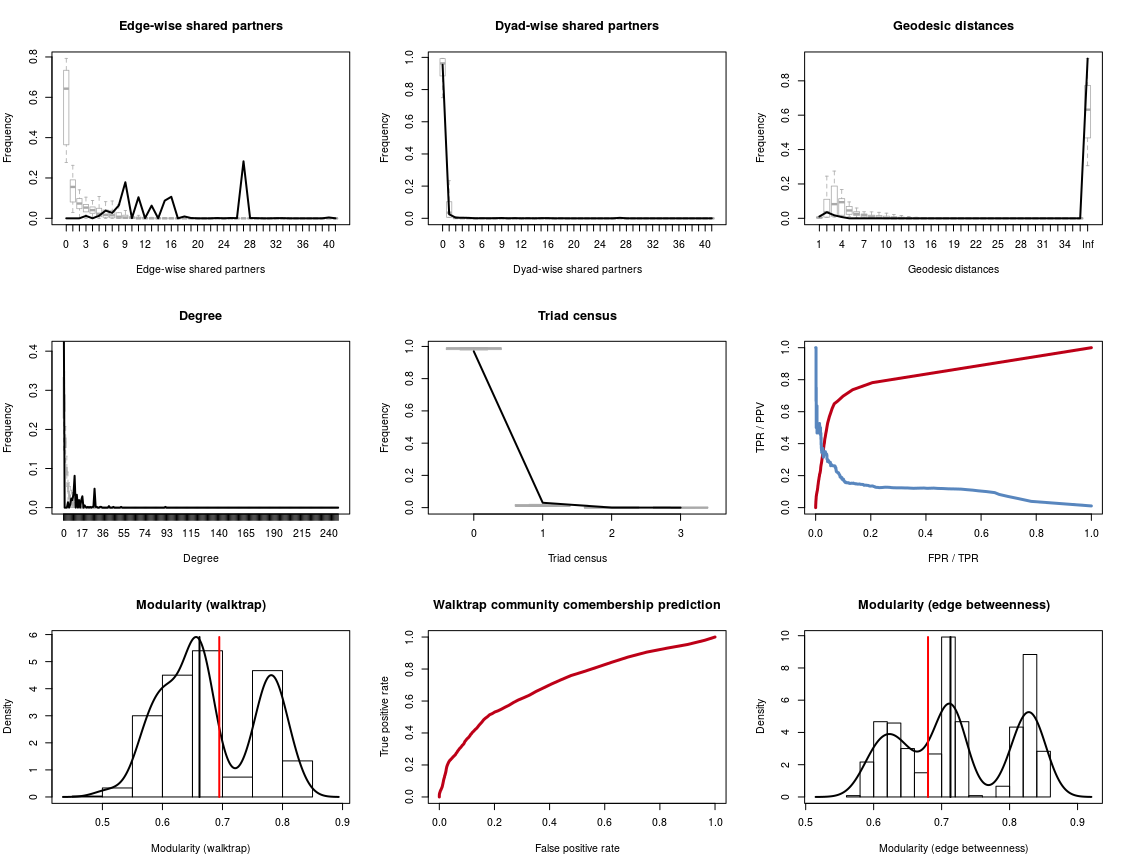
\includegraphics[scale=0.65]{Chapters/hiv/statMod/tergm_gof}
\caption{Goodness-of-fit assessment for the final HIV/AIDS TERGM Model 4 with temporal dependencies of the HIV/AIDS co-authorship network.}
\label{fig:hiv_tergm-gof}
%\end{figure}
\end{sidewaysfigure}

\pagebreak
\subsubsection{Latent Network Model}
\label{hiv_sec:results_lnm}
In figure \ref{fig:hiv_lnm_viz}, we present the 3-dimensional visualization of the HIV/AIDS co-authorship with layouts determined according to the inferred latent eigenvectors from the no pair-specific model (on top), the model containing nodal covariates (middle), and the model containing nodal and dyadic covariates (bottom). Blue vertices represent authors affiliated to Beninese research institutions, Red vertices are authors affiliated to international institutions, Gold vertices represent authors affiliated to African research institutions other than Benin, and White vertices represent authors with no determined affiliations. Vertex sizes are set to be proportional to the betweenness value of each vertex, with bigger vertices emphasizing key broker authors in the network. \\
The first visualization represents the LNM with no pair-specific covariates. It shows mainly two clusters with little demarcation. We can see that there is a heterogeneity in the spatial distribution of the vertices. After adjusting for the nodal covariates (second visualization), the clustering of the nodes appears less apparent. This results seem to suggest the non-significant role of geography in the establishment of collaboration ties in the HIV/AIDS co-authorship network. \\
After adding dyadic variables to the model, the resulting visualization shows that there is less structure left to be captured by the latent variables (bottom subfigure on figure \ref{fig:hiv_lnm_viz}). This observation can explain the failure of our ERGM and TERGM containing dyadic covariates to converge. It also confirms our ERGM and TERGM findings. \\
We assess the goodness-of-fit of the LNMs. The ROC curves on figure \ref{fig:hiv_lnm_roc} shows that the LNM model containing the nodal covariates ($AUC=0.966$) outperforms the null model ($AUC=0.898$).

\begin{figure}[!h]
\center
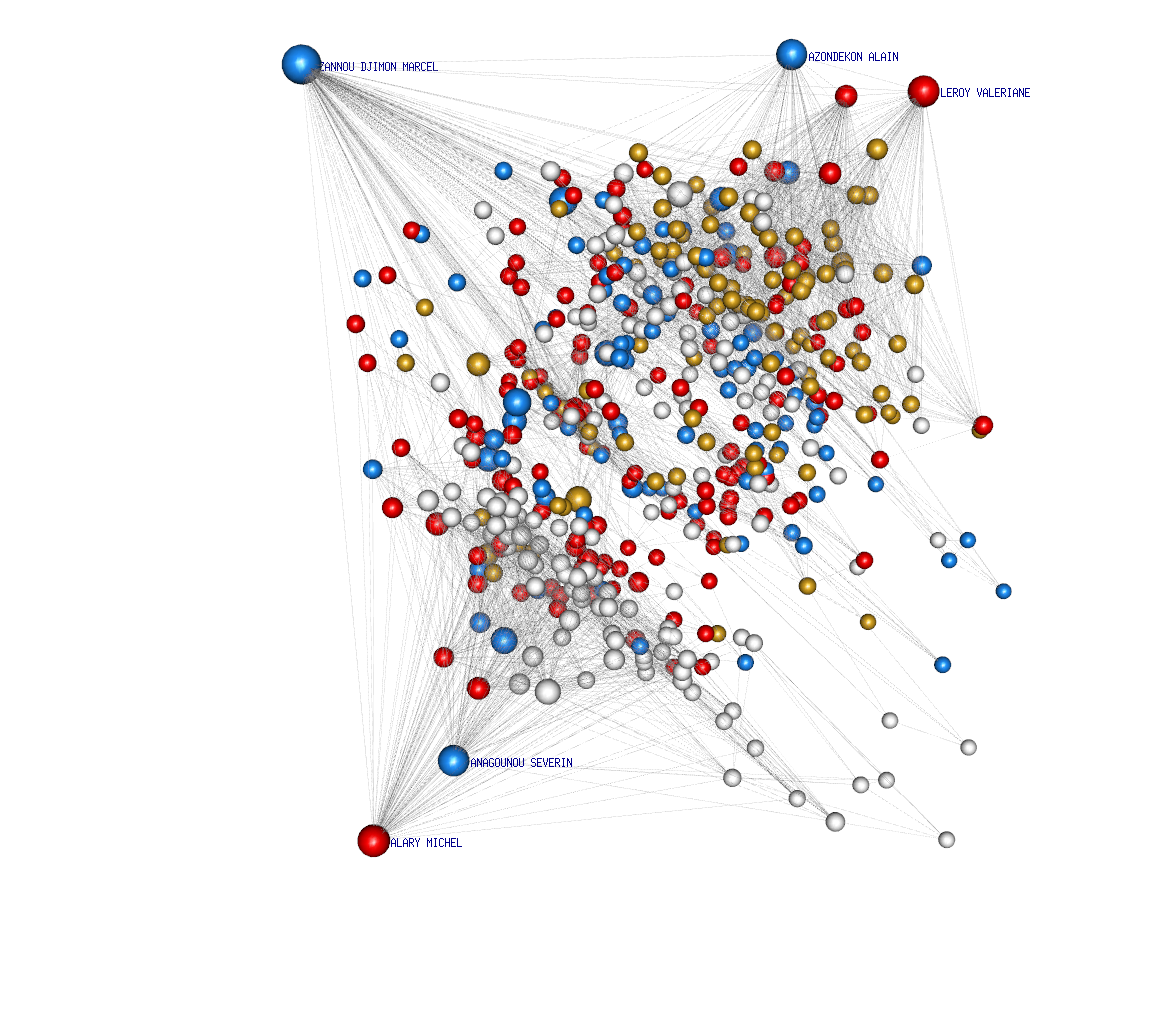
\includegraphics[scale=0.2,trim={5cm 0 0 0}]{Chapters/hiv/statMod/lnm_mod1.png}
\vspace{0px}\\
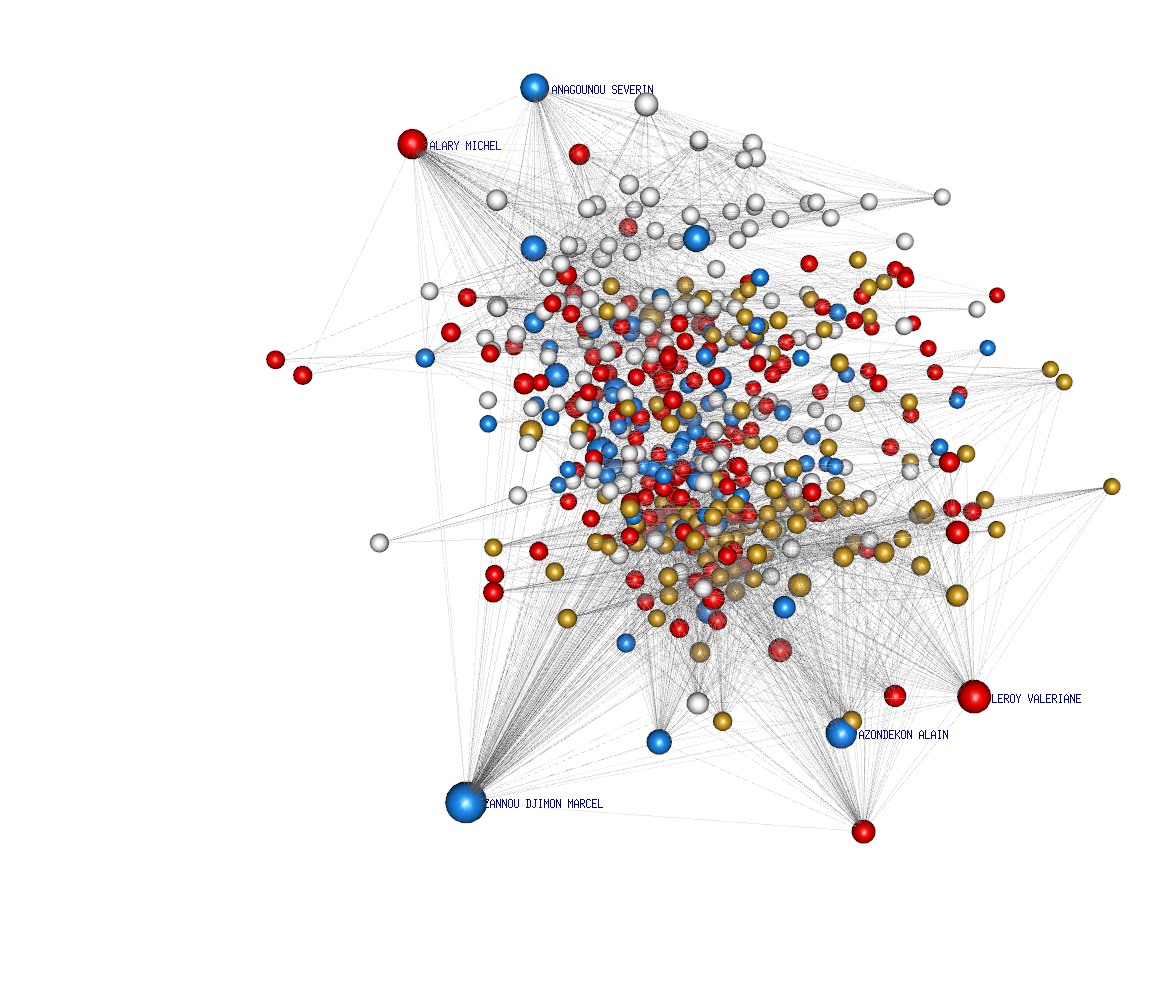
\includegraphics[scale=0.2,trim={5cm 0 0 5cm}]{Chapters/hiv/statMod/lnm_mod4_allNodal.png}
\vspace{2px}\\
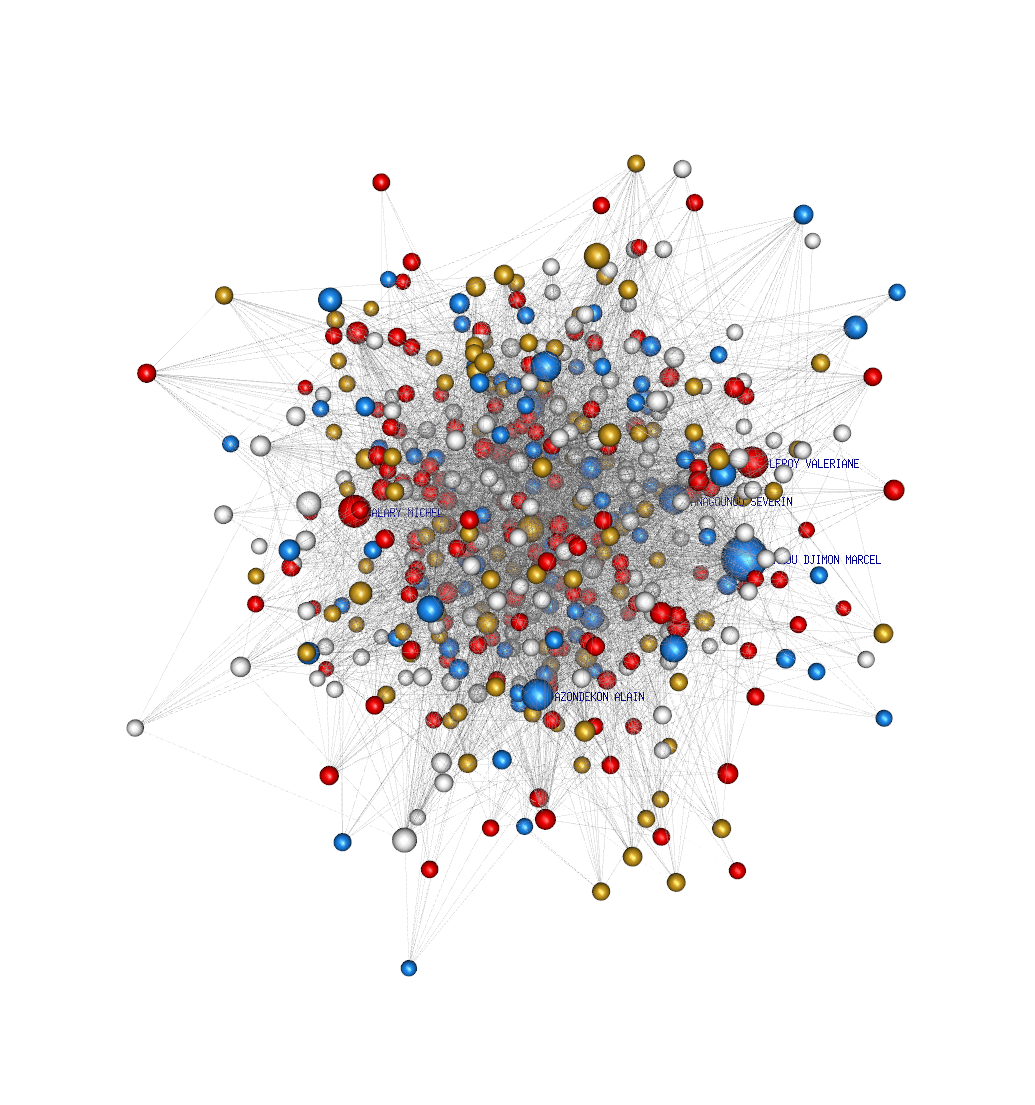
\includegraphics[scale=0.18,trim={5cm 5cm 5cm 5cm}]{Chapters/hiv/statMod/lnm_mod7_allAttributes.png}
\caption{Visualizations of the HIV/AIDS co-authorship network with layouts determined according to the inferred latent eigenvectors in the LNM models (International (Red); Regional (Gold); Local (Blue); Unknown (White)).
% with no pair-specific covariates (top), nodal covariates (middle), and all covariates (bottom).
}
\label{fig:hiv_lnm_viz}
\end{figure}

\begin{figure}[!h]
\centering
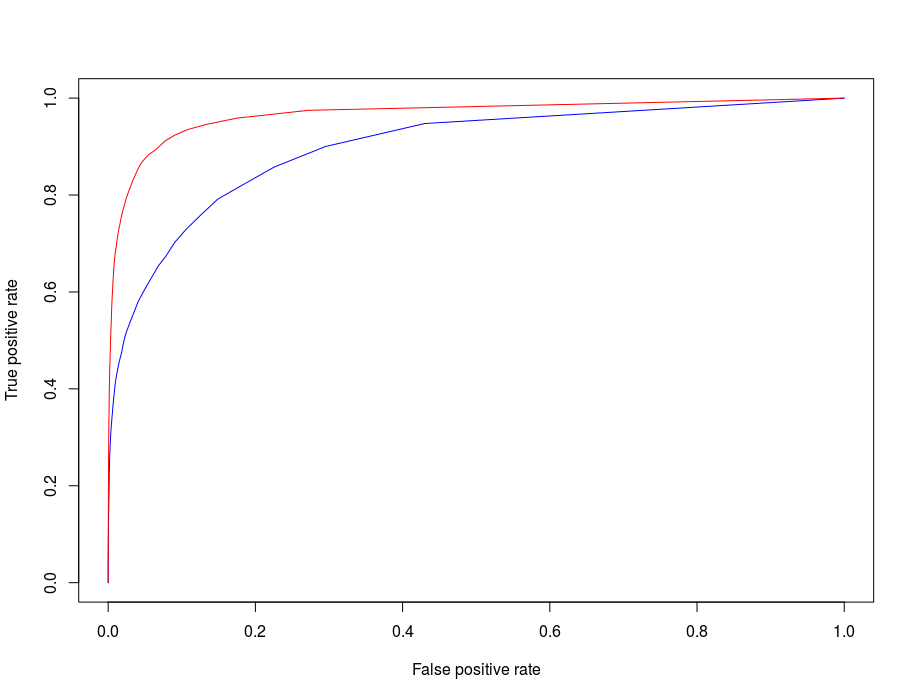
\includegraphics[scale=0.5]{Chapters/hiv/statMod/lnm_ROC_nullVSallNodal.png}
\caption{ROC curves comparing the goodness-of fit of the HIV/AIDS co-authorship network for the model specifying (i) no pair specific covariates (blue) and the model specifying (ii) nodal covariates (red)%, and (iii) nodal and dyadic covariates (green), respectively
.}
\label{fig:hiv_lnm_roc}
\end{figure}~\\~\\

\pagebreak
\section{Discussion and Conclusion}
\label{sec:hiv_discussion}
This chapter deciphers the HIV/AIDS co-authorship network over the last 20 years. The results from the descriptive analyses in this chapter are similar to the descriptive analyses results from chapter \ref{chap:hiv}. Similar to our findings for the malaria co-authorship network, the HIV/AIDS co-authorship network in Benin is a complex network, as it exhibits unexpected properties that are more extreme than the 4 mathematical models used for the Monte-Carlo based simulations. The observed characteristics disproved previous studies supporting the idea that co-authorship have small world properties \cite{gonzalez-alcaide_scientific_2012} or are preferential attachment networks \citep{wagner_network_2005}. In fact, unlike our methodology, those studies mainly used descriptive methods and did not apply advance statistical methods to test their network properties.
The HIV/AIDS co-authorship network in Benin has a low density with a highly right-skewed node degree distribution. Compared to the malaria co-authorship network, the relatively low transitivity provides evidence of less hierarchy - well connected authors in this network tend to connect with poorly connected ones. This also indicates that this network is less assortative than the malaria co-authorship network, with prolific and non tenure authors connected to similar authors.
% clustering coefficient and ANND provide evidence of hierarchy – trade partners of well-connected countries are less interconnected relative to those of poorly connected ones – and is very dissortative – countries holding many trade partners are on average connected with countries holding relatively few countries.
As in Salamati and Soheili \cite{salamati_social_2016}, The flow of information in the HIV/AIDS network in Benin is slow as it only relies on 8 authors representing less than 1\% of all the authors in the network. The removal of these authors from the network would lead to its collapse. Such a structural vulnerability is not just inherent to the HIV/AIDS co-authorship network, as it is a global observation already reported elsewhere \cite{toivanen_african_2011}.  Since the mathematical models applied here, fell short to thoroughly explain the mechanistic phenomenon explaining the growth and the structure of the network, we suspect hidden factors which we attempted to model using advanced statistical models. \\
As our first modeling approach, the SBM identified heterogeneous classes with no dominance of regional, national or international players, despite a reported higher likelihood of Sub-Saharan African countries to collaborate with non-African states \cite{onyancha_knowledge_2011}.\\
Based on the results from our ERGM and TERGM models, in the HIV/AIDS co-authorship network, authors are more likely to establish collaboration ties within their research groups or communities. Unfortunately, we were not able to control for transitivity as all the models adjusting for this term failed to converge. We suspect the size and complexity of this network to have prevented the convergence of such models, even after 1,000 iterations \cite{schmid_exponential_2017}. \\ 
Factors such as number of publications, number of citations and number of collaborations were found to have a small but significant (p<0.001) association with co-authorship, confirming therefore our first hypothesis. Adding temporal dependencies to our ERGM tremendously improved the fitness of the model to the observed network data, but at a cost of decreased performance compared to the model without temporal dependencies.\\
The LNM complements the ERGM and TERGM by adding another layer of analysis. With the LNM, we are able to visualize the effect of geography on the structure of the network. The lack of clear cluster demarcation suggests that distance does not play a significant role in collaboration tie formation in the HIV/AIDS network. \\
Our results confirm that the regain in HIV/AIDS research funding has led to a significant increase in publications number and research collaborations in Benin. In order to consolidate the knowledge generated, there is an urgent need to reinforce the HIV/AIDS research network in Benin given its vulnerability. Identified key brokers and most productive authors need to continuously be supported, and identified junior scientists in the field be promoted.
